\documentclass[a4paper]{scrartcl}
\usepackage[utf8]{inputenc}
\usepackage{tikz}
\usetikzlibrary{trees,shapes}
\usepackage{amsmath}
\usepackage{amssymb}
\usepackage{graphics,color,caption,subcaption}

\begin{document}

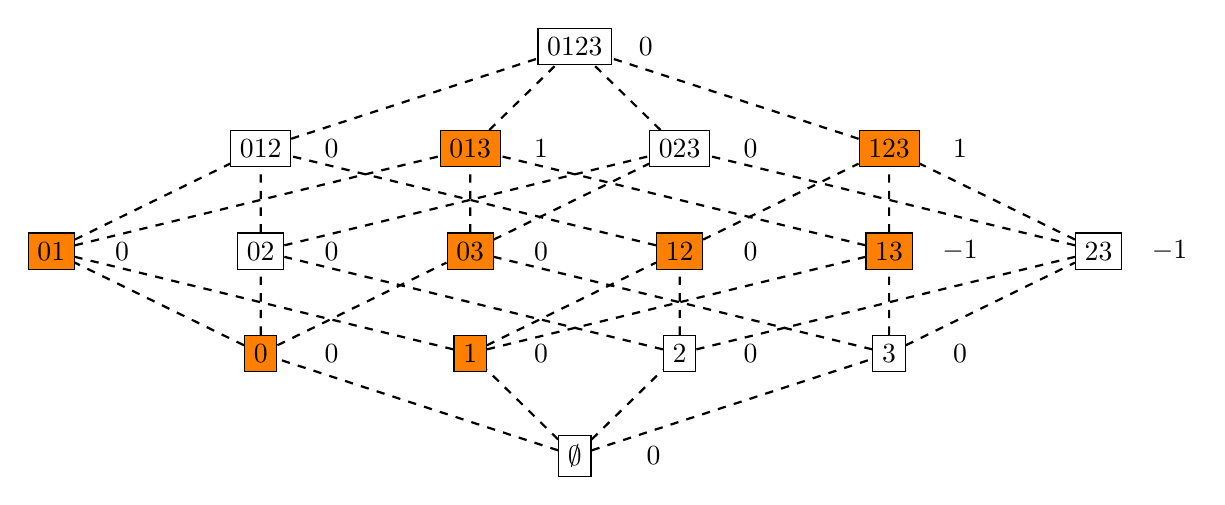
\begin{tikzpicture}[xscale=1.4]
\tikzset{nodestyle/.style={draw,rectangle}}
 ===== NODES ====

  \node[nodestyle] (emptyset) at (0.0, 0.0) {$\emptyset$};
  \node[right of=emptyset] {$0$};
  \node[nodestyle,fill=orange] (0) at (-2.85, 1.3) {$0$};
  \node[right of=0,xshift=-.1cm] {$0$};
  \node[nodestyle,fill=orange] (1) at (-0.95, 1.3) {$1$};
  \node[right of=1,xshift=-.1cm] {$0$};
  \node[nodestyle] (2) at (0.95, 1.3) {$2$};
  \node[right of=2,xshift=-.1cm] {$0$};
  \node[nodestyle] (3) at (2.85, 1.3) {$3$};
  \node[right of=3,xshift=-.1cm] {$0$};
  \node[nodestyle,fill=orange] (01) at (-4.75, 2.6) {$01$};
  \node[right of=01,xshift=-.1cm] {$0$};
  \node[nodestyle] (02) at (-2.85, 2.6) {$02$};
  \node[right of=02,xshift=-.1cm] {$0$};
  \node[nodestyle,fill=orange] (03) at (-0.95, 2.6) {$03$};
  \node[right of=03,xshift=-.1cm] {$0$};
  \node[nodestyle,fill=orange] (12) at (0.95, 2.6) {$12$};
  \node[right of=12,xshift=-.1cm] {$0$};
  \node[nodestyle,fill=orange] (13) at (2.85, 2.6) {$13$};
  \node[right of=13,xshift=-.1cm] {$-1$};
  \node[nodestyle] (23) at (4.75, 2.6) {$23$};
  \node[right of=23,xshift=-.1cm] {$-1$};
  \node[nodestyle] (012) at (-2.85, 3.9) {$012$};
  \node[right of=012,xshift=-.1cm] {$0$};
  \node[nodestyle,fill=orange] (013) at (-0.95, 3.9) {$013$};
  \node[right of=013,xshift=-.1cm] {$1$};
  \node[nodestyle] (023) at (0.95, 3.9) {$023$};
  \node[right of=023,xshift=-.1cm] {$0$};
  \node[nodestyle,fill=orange] (123) at (2.85, 3.9) {$123$};
  \node[right of=123,xshift=-.1cm] {$1$};
  \node[nodestyle] (0123) at (0.0, 5.2) {$0123$};
  \node[right of=0123,xshift=-.1cm] {$0$};


 ===== EDGES ====

\draw[black,thick,dashed] (emptyset) -- (0);
\draw[black,thick,dashed] (emptyset) -- (1);
\draw[black,thick,dashed] (emptyset) -- (2);
\draw[black,thick,dashed] (emptyset) -- (3);
\draw[black,thick,dashed] (0) -- (01);
\draw[black,thick,dashed] (0) -- (02);
\draw[black,thick,dashed] (0) -- (03);
\draw[black,thick,dashed] (1) -- (01);
\draw[black,thick,dashed] (1) -- (12);
\draw[black,thick,dashed] (1) -- (13);
\draw[black,thick,dashed] (2) -- (02);
\draw[black,thick,dashed] (2) -- (12);
\draw[black,thick,dashed] (2) -- (23);
\draw[black,thick,dashed] (3) -- (03);
\draw[black,thick,dashed] (3) -- (13);
\draw[black,thick,dashed] (3) -- (23);
\draw[black,thick,dashed] (01) -- (012);
\draw[black,thick,dashed] (01) -- (013);
\draw[black,thick,dashed] (02) -- (012);
\draw[black,thick,dashed] (02) -- (023);
\draw[black,thick,dashed] (03) -- (013);
\draw[black,thick,dashed] (03) -- (023);
\draw[black,thick,dashed] (12) -- (012);
\draw[black,thick,dashed] (12) -- (123);
\draw[black,thick,dashed] (13) -- (013);
\draw[black,thick,dashed] (13) -- (123);
\draw[black,thick,dashed] (23) -- (023);
\draw[black,thick,dashed] (23) -- (123);
\draw[black,thick,dashed] (012) -- (0123);
\draw[black,thick,dashed] (013) -- (0123);
\draw[black,thick,dashed] (023) -- (0123);
\draw[black,thick,dashed] (123) -- (0123);
\end{tikzpicture}

\end{document}